\documentclass[11pt]{article}

% ---------- Packages ----------
\usepackage[margin=1in]{geometry}
\usepackage{amsmath,amssymb,amsthm}
\usepackage{graphicx}
\usepackage{booktabs}
\usepackage{longtable}
\usepackage{array}
\usepackage{xcolor}
\usepackage{hyperref}
\usepackage{caption}
\usepackage{subcaption}
\usepackage{enumitem}
\usepackage{fancyhdr}
\usepackage{titlesec}
\usepackage{tocloft}
\usepackage[table]{xcolor}

\hypersetup{
  colorlinks=true,
  linkcolor=blue!50!black,
  citecolor=blue!50!black,
  urlcolor=blue!50!black,
}

\definecolor{assumedcolor}{RGB}{178,34,34}
\definecolor{papercolor}{RGB}{0,102,51}
\definecolor{derivedcolor}{RGB}{0,51,153}

\newcommand{\FROMPAPER}{\textcolor{papercolor}{\textbf{[PAPER]}}}
\newcommand{\DERIVED}{\textcolor{derivedcolor}{\textbf{[DERIVED]}}}
\newcommand{\ASSUMED}{\textcolor{assumedcolor}{\textbf{[ASSUMED]}}}

\setlength{\headheight}{14pt}
\pagestyle{fancy}
\fancyhf{}
\fancyhead[L]{GNEP for Competing Plastic-Recycling Agents --- Linear-Cost Interim Draft}
\fancyhead[R]{\thepage}
\renewcommand{\headrulewidth}{0.4pt}

\titleformat{\section}{\normalfont\Large\bfseries}{\thesection}{1em}{}
\titleformat{\subsection}{\normalfont\large\bfseries}{\thesubsection}{1em}{}

\setlength{\cftbeforesecskip}{6pt}

\title{\textbf{A Generalized Nash Equilibrium Model for Competing \\
Plastic-Recycling Agents: Formulation, Parameterization, \\
and Base-Case Results \\[0.3em] \large (Linear-Cost Interim Draft)}}
\author{Technical Report --- Paola\_Game\_Theory project}
\date{\today}

\begin{document}

\maketitle
\thispagestyle{empty}

\vspace{-1em}
\begin{center}
\begin{minipage}{0.92\textwidth}
\small
\textbf{Color key used throughout this report:}\\
\FROMPAPER\ --- value taken directly from Mu\~{n}oz-Briones et al.\ or a table/figure therein.\\
\DERIVED\ --- value recovered from the authors' own underlying model (a Julia/JuMP
notebook and a source spreadsheet feeding the paper) that is not printed in the
paper itself, but is real data, not a guess.\\
\ASSUMED\ --- value with no traceable source in the paper or the authors' data;
a defensible default chosen for this study and flagged for confirmation.

\vspace{0.6em}
\textbf{What this draft is.} This is an \emph{interim} report. Every agent's
operating cost is modeled as \textbf{purely linear} in throughput
(cost $= a_i q_i$, a constant cost per ton) --- nothing convex or
``calibrated'' is involved. A convex refinement is a possible future
extension, mentioned once, at the end (Section~\ref{sec:scope}), and nowhere
else in this document.
\end{minipage}
\end{center}
\vspace{1em}

\tableofcontents
\newpage

% =============================================================================
\section{Problem Statement}
\label{sec:problem}

\subsection{The source paper}

Mu\~{n}oz-Briones, Ikegwu, Martinez, Granger, Van Lehn, Zavala, Huber, and
Avraamidou, \emph{``Decision support for circular economy waste management of
mixed plastic streams: A case study on post-industrial multilayer
films''} (referred to throughout this report as ``the paper''), solves a
\textbf{single-planner, multi-objective mixed-integer nonlinear program
(MINLP)} for the management of 8{,}000 tons/year of post-industrial multilayer
plastic film generated in Wisconsin. A single decision-maker chooses, for the
entire feedstock stream, which technology pathway to route it through ---
solvent-targeted recovery and precipitation (STRAP), incineration,
gasification (three configurations), or landfill --- and in the case of STRAP,
which polymer to remove first and with which solvent. The planner's objective
is one of three criteria evaluated separately: maximize profit, minimize
greenhouse-gas emissions, or maximize a circularity index. The model is a
single centralized optimization: there is one decision-maker and no
competition for feedstock.

\subsection{The extension: from a planner to a market}

This project reformulates the same underlying technologies as a
\textbf{Generalized Nash Equilibrium Problem (GNEP)}. Instead of one planner
routing all 8{,}000 tons, each candidate technology is recast as an
\textbf{independent, self-interested firm} that must \emph{buy} feedstock from
a common, limited pool and decide its own throughput to maximize its own
profit. Three technologies are modeled as competing agents:

\begin{itemize}[leftmargin=2em]
  \item \textbf{S --- STRAP} (solvent-targeted recovery and precipitation),
        internal configuration frozen to the paper's best-performing pathway
        (Section~\ref{sec:strap-config}).
  \item \textbf{W --- Incineration} (waste-to-energy).
  \item \textbf{G --- Gasification} for energy recovery.
\end{itemize}

Landfill is \emph{not} an agent. It appears only in two places: (a) as an
internal residue-disposal cost inside every agent's own objective function
(each agent pays a tipping fee on the fraction of its own feed that it cannot
convert to product), and (b) as the sink for whatever feedstock no agent
chooses to buy, which affects system-wide emissions accounting but never any
agent's profit.

Because all three agents draw from the \emph{same} 8{,}000 t/yr pool, their
individually optimal decisions are coupled through one shared constraint. This
coupling through a shared feasible-region constraint --- rather than through
the agents' objective functions directly --- is precisely what makes the game
\emph{generalized} rather than an ordinary (Nash) game, and it is what this
report's entire mathematical apparatus is built to handle.

\subsection{The central question}

When three firms compete for one limited pool of feedstock, competition
itself implicitly prices that feedstock: every additional ton any one firm
buys is a ton the others cannot have. That implicit price is the
\textbf{shadow price $\lambda$} (USD/ton) on the shared feedstock constraint.
$\lambda$ is never chosen or assumed --- it is an emergent output of the
equilibrium, and it is the headline quantity this entire study is built to
compute. Economically, $\lambda$ acts as a uniform surcharge that every agent
pays on top of its own production costs, driving each firm's optimal
throughput down from what it would choose if feedstock were free and
unlimited.

\subsection{Scope of this report}
\label{sec:scope-report}

This is an \textbf{interim draft} reporting two results, both under a
\textbf{linear} operating-cost structure:
\begin{enumerate}[leftmargin=2em]
  \item The base-case equilibrium at the paper's own feedstock level,
        $Q_{\mathrm{tot}} = 8{,}000$ t/yr (Section~\ref{sec:results-base}).
  \item \textbf{SA-1}: how the equilibrium price $\lambda$ responds to
        feedstock scarcity, sweeping $Q_{\mathrm{tot}}$ from $0$ to
        $18{,}000$ t/yr (Section~\ref{sec:results-sa1}).
\end{enumerate}
Further sensitivity work (whether the assumed capacities are themselves
defensible, and how much the most load-bearing assumed parameters move the
headline number) and a convex-cost refinement are possible future extensions,
noted at the end, in Section~\ref{sec:scope}.

\textbf{Explicitly out of scope} for this version of the model itself (not
just this draft): output-price coupling (all prices are fixed), cost coupling
(e.g.\ a landfill fee that depends on total system-wide residue volume), an
emissions cap, and any genuine two-stage (endogenous-capacity) equilibrium.
These are deliberate boundaries, not oversights, and are revisited in
Section~\ref{sec:scope}.


% =============================================================================
\section{Mathematical Formulation}
\label{sec:formulation}

\subsection{Sets and indices}

\begin{center}
\begin{tabular}{@{}ll@{}}
\toprule
Symbol & Meaning \\
\midrule
$i \in \{S, W, G\}$ & Agent index: STRAP, Incineration, Gasification \\
$k$ & Product index (agent-specific; see Table~\ref{tab:products}) \\
\bottomrule
\end{tabular}
\end{center}

\subsection{STRAP's frozen internal configuration}
\label{sec:strap-config}

STRAP's process design is a superstructure in the paper: which polymer to
remove in which wash, with which solvent, is itself a decision. For this GNEP,
STRAP's internal configuration is \textbf{fixed} to the paper's own
best-performing (highest-profit) pathway, so that STRAP's problem reduces to a
single continuous decision (how much feedstock to buy) with no internal
binary variables:

\begin{itemize}[leftmargin=2em]
  \item Wash 1: remove PE using tetrachloroethylene (PCE).
  \item Wash 2: remove EVOH using $\gamma$-butyrolactone.
  \item Overall yield: 97\%.
\end{itemize}

This choice is essential to the model's tractability: with no binary
variables anywhere in the game, every agent's optimization problem is smooth,
which is what makes stacking Karush--Kuhn--Tucker (KKT) conditions across
agents (Section~\ref{sec:kkt}) a valid solution method.

\subsection{Decision variables}

Per agent $i$, the only free decision is
\[
q_i \geq 0 \quad \text{[ton/yr]} \qquad \text{--- feedstock purchased and processed by agent } i.
\]
Every other quantity --- product outputs, residue, emissions --- is
\textbf{affine in $q_i$} and is declared as an explicit variable with its own
defining constraint (rather than pre-substituted away), so the model structure
generalizes cleanly to later extensions:
\begin{align}
  y_{ik} &= \eta_{ik}\, q_i &&\text{[product-$k$ units/yr]} \label{eq:yield}\\
  r_i &= \rho_i\, q_i &&\text{[ton/yr, residue to landfill]} \label{eq:residue}\\
  E_i &= e_i\, q_i &&\text{[t CO$_2$e/yr, reported only, never constrained]} \label{eq:emissions}
\end{align}
where $\eta_{ik}$ is the yield of product $k$ per ton of feedstock processed
by agent $i$, $\rho_i$ is agent $i$'s residue fraction, and $e_i$ is agent
$i$'s total emission factor (process emissions plus the emissions of
landfilling its own residue).

\subsection{Agent $i$'s optimization problem}
\label{sec:agent-problem}

Each agent solves a profit-maximization problem over its own throughput
$q_i$, taking the (yet unknown) shared feedstock price $\lambda$ as given.
Operating cost is \textbf{linear} in throughput: $a_i$ is a constant cost per
ton (Section~\ref{sec:opex}), so total operating cost is simply $a_i q_i$.
\begin{align}
\max_{q_i \geq 0} \quad
\pi_i \;=\;& \underbrace{\sum_k P_k\, \eta_{ik}\, q_i}_{\text{revenue}}
\;-\; \underbrace{a_i\, q_i}_{\text{operating cost}}
\;-\; \underbrace{p_{\mathrm{raw}}\, q_i}_{\text{feedstock cost}} \notag \\
&\;-\; \underbrace{c_{\mathrm{lf}}\, \rho_i\, q_i}_{\text{residue disposal}}
\;-\; \underbrace{\mathrm{ACC}_i}_{\text{annualized CAPEX (constant)}}
\label{eq:objective}
\end{align}
subject to
\begin{align}
  q_i &\leq \mathrm{Cap}_i && \text{(private capacity bound; multiplier } \mu_i \text{)} \label{eq:privatecon}\\
  \sum_{j \in \{S,W,G\}} q_j &\leq Q_{\mathrm{tot}} && \text{(\textbf{shared} feedstock pool; multiplier } \lambda \text{)} \label{eq:sharedcon}
\end{align}
where $P_k$ is the fixed market price of product $k$ (USD per product unit),
$p_{\mathrm{raw}}$ is the price paid per ton of feedstock, $c_{\mathrm{lf}}$
is the landfill tipping fee paid on the agent's own residue, and
$\mathrm{ACC}_i$ is the annualized capital charge --- a constant that does
\emph{not} affect the equilibrium throughput $q_i^\ast$, but does determine
whether the agent is economically viable net of capital.

\subsection{Net margin}
\label{sec:margin}

Collect every constant per-ton term of Eq.~\eqref{eq:objective} into one
number:
\begin{equation}
m_i \;\equiv\; \sum_k P_k\, \eta_{ik} \;-\; a_i \;-\; p_{\mathrm{raw}} \;-\; c_{\mathrm{lf}}\,\rho_i
\qquad \text{[USD/ton]}
\label{eq:margin}
\end{equation}
$m_i$ is agent $i$'s profit per additional ton of feedstock, and --- because
cost is linear --- it is a \emph{constant}: the same number at every
throughput level, not just near zero. $\pi_i$ then reduces to
$\pi_i = m_i q_i - \mathrm{ACC}_i$, an affine (straight-line) function of
$q_i$. $m_i$ is the single number that ranks the agents' willingness to pay
for feedstock.

\subsection{The shared constraint and the Variational Equilibrium}

Because constraint~\eqref{eq:sharedcon} is shared by all three agents, this is
a \emph{Generalized} Nash game: each agent's own feasible region depends on
what the \emph{others} choose. Such games generally admit infinitely many
Generalized Nash Equilibria (GNE), each corresponding to a different way of
splitting the shared resource, and each potentially supported by a
\emph{different} multiplier on the shared constraint for each agent.

This study solves for the \textbf{Variational Equilibrium (VE)}: the
refinement of GNE in which \emph{every agent faces the same multiplier
$\lambda$} on the shared constraint. Economically, this is the natural
solution concept for a competitive market: $\lambda$ is a single, uniform
market-clearing price that every buyer faces identically, exactly as a real
commodity market would produce.

\subsection{Stacked KKT / complementarity system}
\label{sec:kkt}

Because $\pi_i$ is affine (hence concave, though not \emph{strictly}
concave) in $q_i$, its Karush--Kuhn--Tucker conditions are still necessary
and sufficient for its own optimum given $\lambda$. Stacking all three
agents' KKT conditions together with the complementarity condition on the
shared constraint gives one square Mixed Complementarity Problem (MCP):
\begin{align}
0 \;\leq\; q_i \;\perp\; \lambda + \mu_i - m_i &\;\geq\; 0
  \qquad \forall i \in \{S,W,G\} \label{eq:kkt-q}\\
0 \;\leq\; \mu_i \;\perp\; \mathrm{Cap}_i - q_i &\;\geq\; 0
  \qquad \forall i \in \{S,W,G\} \label{eq:kkt-mu}\\
0 \;\leq\; \lambda \;\perp\; Q_{\mathrm{tot}} - \sum_j q_j &\;\geq\; 0 \label{eq:kkt-lambda}
\end{align}
where $a \perp b$ denotes the complementarity condition $a \cdot b = 0$. Note
condition~\eqref{eq:kkt-q}: the stationarity term $\lambda + \mu_i - m_i$
does \emph{not} depend on $q_i$ --- a direct consequence of linear cost. This
is what makes the best response a step function rather than a smooth curve,
worked out next.

\subsection{Best response, and the tie case}
\label{sec:bestresponse}

Because $\lambda + \mu_i - m_i$ is constant in $q_i$, an unconstrained agent's
profit $m_i q_i$ is monotonic in $q_i$ with no interior optimum: the agent
wants either \emph{all} the feedstock it can get, or \emph{none}.
Concretely, at a candidate price $\lambda$:
\begin{equation}
q_i(\lambda) \;=\;
\begin{cases}
\mathrm{Cap}_i & m_i > \lambda \quad \text{(wants strictly more; capacity binds)} \\
0 & m_i < \lambda \quad \text{(priced out)} \\
\text{any value in } [0, \mathrm{Cap}_i] & m_i = \lambda \quad \text{(exactly indifferent)}
\end{cases}
\label{eq:bestresponse}
\end{equation}
The third case is the only subtlety linear cost introduces: at the one price
where an agent's margin exactly equals $\lambda$, \emph{every} throughput is
equally profitable for that agent, so its own optimization alone does not
pin down a quantity. What \emph{does} pin it down is the shared constraint:
whichever agent is on the margin is handed exactly the residual feedstock
needed to make $\sum_i q_i = Q_{\mathrm{tot}}$ --- the standard economic
convention for a marginal price-setting supplier under constant marginal
cost. See Section~\ref{sec:results-base} for exactly this happening in the
base case.

\subsection{Equilibrium states}
\label{sec:equilibrium-states}

At any solved equilibrium, each agent occupies exactly one of three
mutually exclusive states, determined by \emph{where it actually sits}, never
by a static property of its own cost alone:
\begin{center}
\begin{tabular}{@{}lll@{}}
\toprule
State & Condition & Economic meaning \\
\midrule
\textsc{At Capacity} & $q_i = \mathrm{Cap}_i,\ \mu_i > 0$ & Wants more feedstock, cannot have it \\
\textsc{Price-Setter} & $0 < q_i < \mathrm{Cap}_i,\ \mu_i = 0$ & On the margin; $m_i = \lambda$ pins the price \\
\textsc{Priced Out} & $q_i = 0,\ m_i < \lambda$ & Cannot outbid the others for a single ton \\
\bottomrule
\end{tabular}
\end{center}
At any given $Q_{\mathrm{tot}}$, at most one agent is normally the
Price-Setter --- it is that agent's own tie condition $m_i = \lambda$ that
determines the market-clearing price for \emph{everyone}, since a common
$\lambda$ is exactly what makes the equilibrium variational.

\subsection{Emissions accounting}

Total system emissions include every agent's own process-plus-residue
emissions \emph{and} the emissions of landfilling whatever feedstock no agent
buys:
\begin{equation}
E_{\mathrm{system}} \;=\; \sum_i e_i\, q_i^\ast \;+\; g_{\mathrm{lf}}\,\big(Q_{\mathrm{tot}} - \textstyle\sum_i q_i^\ast\big)
\label{eq:sysemissions}
\end{equation}

\subsection{Solving for the equilibrium}
\label{sec:methods}

Because every agent's best response is the step function of
Eq.~\eqref{eq:bestresponse}, the equilibrium does not require an iterative
numerical solver here: rank the three agents by margin $m_i$ (descending),
and hand each one its full capacity in that order until $Q_{\mathrm{tot}}$
is exhausted. The last agent whose capacity is only \emph{partially} used is
the Price-Setter, and $\lambda$ equals its margin $m_i$. Section
\ref{sec:results-base} carries this out explicitly for the base case.


% =============================================================================
\section{Parameters}
\label{sec:parameters}

\subsection{Feedstock composition and base-case availability}

\begin{center}
\begin{tabular}{@{}lp{6.3cm}rl@{}}
\toprule
Symbol & Description & Value & Source \\
\midrule
$Q_{\mathrm{tot}}^{\mathrm{base}}$ & Base-case feedstock availability & $8{,}000$ ton/yr & \FROMPAPER \\
$f_{\mathrm{PE}}$ & Feedstock mass fraction, PE & $0.60$ & \FROMPAPER \\
$f_{\mathrm{PET}}$ & Feedstock mass fraction, PET & $0.20$ & \FROMPAPER \\
$f_{\mathrm{N6}}$ & Feedstock mass fraction, N6 (nylon) & $0.10$ & \FROMPAPER \\
$f_{\mathrm{EVOH}}$ & Feedstock mass fraction, EVOH & $0.10$ & \FROMPAPER \\
\bottomrule
\end{tabular}
\end{center}

PET and N6 are \emph{not} recoverable by STRAP under the frozen configuration
(Section~\ref{sec:strap-config}): the paper states no solvent pair exists to
separate a PET/N6 film, so that fraction of any STRAP-processed ton leaves as
residue.

\subsection{STRAP (agent S)}
\label{sec:strap-params}

\begin{center}
\begin{tabular}{@{}lp{6.3cm}rl@{}}
\toprule
Symbol & Description & Value & Source \\
\midrule
$\eta_{\mathrm{yield}}$ & Overall STRAP yield & $0.97$ & \FROMPAPER \\
$P_{\mathrm{PE}}$ & Recycled PE resin price & $1{,}173$ USD/ton & \FROMPAPER \\
$P_{\mathrm{EVOH}}$ & Recycled EVOH resin price & $8{,}100$ USD/ton & \FROMPAPER \\
$\eta_{S,\mathrm{PE}}$ & PE yield per ton feed ($=\eta_{\mathrm{yield}} f_{\mathrm{PE}}$) & $0.582$ ton/ton & \DERIVED \\
$\eta_{S,\mathrm{EVOH}}$ & EVOH yield per ton feed ($=\eta_{\mathrm{yield}} f_{\mathrm{EVOH}}$) & $0.097$ ton/ton & \DERIVED \\
$\mathrm{REV}_S$ & Gross revenue per ton feed & $1{,}468.386$ USD/ton & \DERIVED \\
$\rho_S$ & Residue fraction ($=1-\eta_{\mathrm{yield}}(f_{\mathrm{PE}}+f_{\mathrm{EVOH}})$) & $0.321$ ton/ton & \DERIVED \\
$\mathrm{CAPEX}_S$ & Total installed capital (wash 1 + wash 2 + shredder) & $53{,}645{,}274$ USD & \DERIVED \\
$\mathrm{OPEX}_S^{\mathrm{ref}}$ & Total operating cost at 8{,}000 t/yr reference basis & $2{,}490{,}259$ USD/yr & \DERIVED \\
$e_{\mathrm{proc},S}$ & Process emission factor & $1.194$ tCO$_2$e/ton & \DERIVED \\
$\mathrm{Cap}_S$ & Nameplate capacity & $6{,}000$ ton/yr & \ASSUMED \\
\bottomrule
\end{tabular}
\end{center}

\subsubsection*{Provenance detail: STRAP's CAPEX and OPEX}
The paper itself prints no installed-cost or operating-cost figures for
STRAP. These were recovered from the authors' own underlying BioSTEAM process
simulation data (a Julia/JuMP notebook and its source spreadsheet, which feed
the paper but are not printed in it), for the paper's best pathway (PE via
PCE in wash 1, EVOH via $\gamma$-butyrolactone in wash 2), Energy Supply
Scenario 1:
\[
\mathrm{CAPEX}_S = \underbrace{35{,}957{,}532}_{\text{wash 1, PE/PCE}}
+ \underbrace{14{,}557{,}669}_{\text{wash 2, EVOH/GBL}}
+ \underbrace{3{,}130{,}073}_{\text{shredder}}
\;=\; 53{,}645{,}274 \text{ USD}
\]
\[
\mathrm{OPEX}_S^{\mathrm{ref}} = \underbrace{941{,}557}_{\text{wash 1}}
+ \underbrace{479{,}709}_{\text{wash 2}}
+ \underbrace{1{,}068{,}992}_{\text{shredder}}
\;=\; 2{,}490{,}259 \text{ USD/yr, at 8{,}000 t/yr}
\]
The process emission factor is likewise built from the per-resin BioSTEAM
GWP factors ($1.1326$ tCO$_2$e/ton PE resin, $2.1661$ tCO$_2$e/ton EVOH
resin, $0.5575$ tCO$_2$e/ton resin for the shredder), scaled to the
$4{,}656$ ton/yr of PE and $776$ ton/yr of EVOH actually recovered at the
8{,}000 t/yr basis, and divided back onto a per-ton-of-feed basis:
$e_{\mathrm{proc},S} = 1.194$ tCO$_2$e/ton feed.

\subsection{Incineration (agent W)}
\label{sec:incineration-params}

\begin{center}
\begin{tabular}{@{}lp{6.3cm}rl@{}}
\toprule
Symbol & Description & Value & Source \\
\midrule
$\mathrm{REV}_W$ & Revenue (energy product value) per ton feed & $259.57$ USD/ton & \DERIVED \\
$\rho_W$ & Residue (ash) fraction & $0.15$ ton/ton & \ASSUMED \\
$e_{\mathrm{proc},W}$ & Process emission factor & $2.38$ tCO$_2$e/ton & \DERIVED \\
$\mathrm{Cap}_W$ & Nameplate capacity & $4{,}000$ ton/yr & \ASSUMED \\
$\mathrm{OPEX}_W^{\mathrm{ref}}$ & Operating cost per ton & $75$ USD/ton & \ASSUMED \\
$\mathrm{CAPEX}_W$ & Installed capital at $\mathrm{Cap}_W$ & $30{,}000{,}000$ USD & \ASSUMED \\
\bottomrule
\end{tabular}
\end{center}

\subsubsection*{Provenance detail: incineration}
The paper never models incineration as a facility anyone owns and operates
--- it is treated purely as a \emph{third-party off-take market}: the
planner sells waste to incineration for $110$ USD/ton
(\texttt{Cgas\_pw} in the authors' notebook), and the authors' spreadsheet
records incineration OPEX and CAPEX as literally zero. Because this GNEP
requires incineration to be an operating firm, its \textbf{revenue} was taken
as $\mathrm{REV}_W = 259.57$ USD/ton (\texttt{Cwte}, the authors' own figure
for ``cost of the product'' --- i.e.\ the value of the electricity/heat sold
--- listed alongside the STRAP resin prices in the same table), while its
\textbf{operating cost} has \emph{no} basis in the paper or the authors' data
at all and was assumed at $75$ USD/ton, a mid-range figure for US
municipal-solid-waste waste-to-energy O\&M (typical range 60--90 USD/ton).
This is flagged as Question 1 and Question 2 for Paola
(Section~\ref{sec:questions}), since incineration turns out to be the agent
that \emph{sets} the equilibrium price at the base case
(Section~\ref{sec:results-base}).

\subsection{Gasification for energy recovery (agent G)}
\label{sec:gasification-params}

\begin{center}
\begin{tabular}{@{}lp{6.3cm}rl@{}}
\toprule
Symbol & Description & Value & Source \\
\midrule
$\mathrm{REV}_G$ & Revenue (heat + electricity) per ton feed & $147.98$ USD/ton & \DERIVED \\
$\rho_G$ & Residue (ash/char) fraction & $0.08$ ton/ton & \ASSUMED \\
$e_{\mathrm{proc},G}$ & Process emission factor & $1.07$ tCO$_2$e/ton & \DERIVED \\
$\mathrm{Cap}_G$ & Nameplate capacity & $4{,}000$ ton/yr & \ASSUMED \\
$\mathrm{OPEX}_G^{\mathrm{ref}}$ & Operating cost per ton & $159.87$ USD/ton & \DERIVED \\
\bottomrule
\end{tabular}
\end{center}

\subsubsection*{Provenance detail: gasification revenue}
$\mathrm{REV}_G$ is built directly from the authors' own product yields and
prices for gasification-for-energy-recovery:
\[
\mathrm{REV}_G = \underbrace{583.33\ \tfrac{\text{MJ}}{\text{ton}} \times 0.13\ \tfrac{\text{USD}}{\text{MJ}}}_{\text{heat}}
+ \underbrace{724.3693\ \tfrac{\text{kWh}}{\text{ton}} \times 0.0996\ \tfrac{\text{USD}}{\text{kWh}}}_{\text{electricity}}
= 147.98 \text{ USD/ton}
\]
Two of the underlying inputs are dimensionally suspect --- the heat price
of $0.13$ USD/MJ ($=130$ USD/GJ) is roughly an order of magnitude above
typical industrial heat prices (5--15 USD/GJ), and the heat yield of
$583$ MJ/tonne is far below the heating value of plastic waste (30--40
GJ/tonne) --- but both are used unmodified since they are the authors' own
figures. The two suspected errors push revenue in opposite directions (a lower
heat price reduces it, a higher heat yield raises it), so the net effect of
correcting them cannot be signed in advance. This is Question~10.

\subsection{Gasification CAPEX scaling}
\label{sec:gcapex}

The authors' own notebook hard-codes gasification-for-energy-recovery
annualized CAPEX at four discrete capacities. Fitting a six-tenths power law
$\mathrm{CAPEX}_G(\mathrm{Cap}) = A\, \mathrm{Cap}^{n}$ to two of these points
gives $n = 0.6000$, $A = 15{,}749.6$, and this fit reproduces the other two
authors' data points to within $0.1\%$:
\begin{center}
\begin{tabular}{@{}rrrr@{}}
\toprule
Capacity (t/yr) & Authors' value (USD/yr) & Fitted value (USD/yr) & Error \\
\midrule
2{,}400 & 1{,}680{,}303 & 1{,}679{,}096 & 0.07\% \\
3{,}200 & 1{,}996{,}874 & (fit point) & --- \\
7{,}200 & 3{,}248{,}331 & (fit point) & --- \\
8{,}000 & 3{,}460{,}308 & 3{,}459{,}341 & 0.03\% \\
\bottomrule
\end{tabular}
\end{center}
Note that this column is already headed ``CAPEX [USD/yr]'' in the authors'
own spreadsheet --- it is \emph{already annualized}, so the capital recovery
factor $\mathrm{CRF}$ is \textbf{not} applied a second time for gasification,
unlike for STRAP and incineration.

\subsection{Shared market and cost parameters}

\begin{center}
\begin{tabular}{@{}lp{6.3cm}rl@{}}
\toprule
Symbol & Description & Value & Source \\
\midrule
$p_{\mathrm{raw}}$ & Feedstock purchase price & $0$ USD/ton & \ASSUMED \\
$c_{\mathrm{lf}}$ & Landfill tipping fee & $60$ USD/ton & \ASSUMED \\
$\mathrm{CRF}$ & Capital recovery factor (10\%, 20 yr) & $0.1175$ /yr & \ASSUMED \\
$g_{\mathrm{lf}}$ & Landfill emission factor ($0.0816$ plus a 9.2-mile haul) & $0.0865$ tCO$_2$e/ton & \DERIVED \\
\bottomrule
\end{tabular}
\end{center}

\paragraph{$p_{\mathrm{raw}}$.} The paper hands its single planner 8{,}000
t/yr of feedstock at zero cost, so there is nothing to extract; $p_{\mathrm{raw}}=0$
is chosen for consistency with the paper. The authors' own model implicitly
values this waste at $110$ USD/ton in a different context (the incineration
transfer price, \texttt{Cgas\_pw}); post-industrial waste can plausibly carry
a \emph{negative} price in reality (the generator pays to have it hauled
away).

\paragraph{$c_{\mathrm{lf}}$.} A representative Wisconsin municipal
solid-waste landfill gate rate. Held \emph{fixed}, i.e.\ not a function of
total system-wide residue volume. The authors' own spreadsheet implies a
landfill cost of only $7.836$ USD/ton, roughly $8\times$ below real Wisconsin
gate rates, and is retained in the code as a cross-check constant.

\paragraph{$\mathrm{CRF}$.} A conventional 10\% discount rate, 20-year asset
life, computed as $\mathrm{CRF} = i(1+i)^n/[(1+i)^n-1]$. The paper's own
convention is undiscounted straight-line annualization over 20 years
($\mathrm{CRF}^{\mathrm{paper}} = 0.05$), retained in the code as a
cross-check constant. This choice affects only which agents are
\emph{viable} net of capital; it never affects the equilibrium throughput
$q_i^\ast$ or $\lambda$ (Eq.~\eqref{eq:objective} shows $\mathrm{ACC}_i$ is a
pure constant in the objective).

\subsection{Operating cost per agent}
\label{sec:opex}

$a_i$ (Eq.~\eqref{eq:objective}) is each agent's operating cost per ton of
feedstock processed. It is read off directly, with no modeling step in
between:
\begin{itemize}[leftmargin=2em]
  \item \textbf{Incineration and gasification:} $\mathrm{OPEX}_i^{\mathrm{ref}}$
        (Sections~\ref{sec:incineration-params}--\ref{sec:gasification-params})
        is already reported per ton, so $a_W = 75.00$ and $a_G = 159.87$
        USD/ton, used as-is.
  \item \textbf{STRAP:} $\mathrm{OPEX}_S^{\mathrm{ref}} = 2{,}490{,}259$
        USD/yr is a total cost at a reference throughput of $q_S^{\mathrm{ref}}
        = 8{,}000$ t/yr (Section~\ref{sec:strap-params}), so
        $a_S = \mathrm{OPEX}_S^{\mathrm{ref}} / q_S^{\mathrm{ref}} = 311.28$
        USD/ton --- a unit conversion (total cost $\div$ throughput), not an
        assumption or a fitted parameter.
\end{itemize}
No other number enters $a_i$. Table~\ref{tab:agents} collects the
result.

\begin{table}[h]
\centering
\caption{Operating cost and net margin per agent, base-case capacities.}
\label{tab:agents}
\begin{tabular}{@{}lrrrrrrr@{}}
\toprule
$i$ & $\mathrm{Cap}_i$ & $\mathrm{REV}_i$ & $a_i$ & $m_i$ & $\rho_i$ & $e_i^{\mathrm{tot}}$ & $\mathrm{ACC}_i$ \\
 & [t/yr] & [USD/t] & [USD/t] & [USD/t] & [t/t] & [tCO$_2$e/t] & [USD/yr] \\
\midrule
S & 6{,}000 & 1{,}468.39 & 311.28 & 1{,}137.84 & 0.321 & 1.221 & 6{,}303{,}320 \\
W & 4{,}000 & 259.57 & 75.00 & 175.57 & 0.150 & 2.393 & 3{,}525{,}000 \\
G & 4{,}000 & 147.98 & 159.87 & $-16.69$ & 0.080 & 1.077 & 2{,}282{,}998 \\
\bottomrule
\end{tabular}
\end{table}

Note the ranking $m_S \gg m_W > 0 > m_G$: gasification's margin is
\textbf{negative} under this linear cost. It costs more, on average, to run
gasification than the energy it produces is worth, so gasification would not
want to operate at \emph{any} feedstock price $\lambda \geq 0$ --- this is a
direct, unavoidable reading of the raw numbers in
Section~\ref{sec:gasification-params}, not an artifact of anything in this
document.

\subsection{Products}

\begin{table}[h]
\centering
\caption{Products sold by each agent, with prices $P_k$ and yields $\eta_{ik}$.}
\label{tab:products}
\begin{tabular}{@{}lp{5.6cm}rrl@{}}
\toprule
Agent & Product $k$ & $P_k$ & $\eta_{ik}$ & Unit \\
\midrule
S & Recycled PE resin & 1{,}173 USD/ton & 0.582 & ton product / ton feed \\
S & Recycled EVOH resin & 8{,}100 USD/ton & 0.097 & ton product / ton feed \\
W & Electricity + heat & 259.57 USD/ton feed & 1.000 & --- (lumped) \\
G & Exported heat & 0.13 USD/MJ & 583.33 & MJ / ton feed \\
G & Exported electricity & 0.0996 USD/kWh & 724.37 & kWh / ton feed \\
\bottomrule
\end{tabular}
\end{table}

\subsection{Emissions unit note}

The paper's Table 8 reports the landfill-only pathway's emissions as
``652.80 kg CO$_2$-eq/year'' against 8{,}000 t/yr of feedstock --- i.e.\
$\approx\!1.9$ kg CO$_2$ per tonne of plastic, roughly 1{,}000$\times$ below
standard plastic-waste LCA figures (incineration alone is typically 2--3
\emph{tonnes} CO$_2$ per tonne of plastic). Tracing this to its source shows
it is a \textbf{table label error, not a data error}: the underlying factor
is $g_{\mathrm{lf}} = 0.0816$ tCO$_2$e/ton, and
$0.0816 \times 8{,}000 = 652.80$ reproduces the paper's number exactly ---
the data is genuinely in \emph{tonnes}, and the paper's column header should
read ``t CO$_2$-eq/yr,'' not ``kg.'' This is corroborated by the paper's own
Table 6, which gives an emissions upper bound of $21{,}303.36$
\emph{tonCO2eq}, the same order of magnitude as the Table 8 entries. No
1{,}000$\times$ correction is applied anywhere in this model; the unit-scale
parameter $\mathrm{EMIS\_UNIT\_SCALE}$ is retained at $1.0$.


% =============================================================================
\section{Results}
\label{sec:results}

\subsection{Base-case equilibrium}
\label{sec:results-base}

At $Q_{\mathrm{tot}} = 8{,}000$ t/yr, rank the agents by margin
(Table~\ref{tab:agents}): $m_S = 1{,}137.84 \gg m_W = 175.57 \gg m_G =
-16.69$. Fill capacity in that order:
\begin{itemize}[leftmargin=2em]
  \item STRAP takes its full capacity, $6{,}000$ t/yr (it would take more
        if it could).
  \item That leaves $8{,}000 - 6{,}000 = 2{,}000$ t/yr, well inside
        incineration's $4{,}000$ t/yr capacity --- so incineration is
        exactly on the margin: it is handed the residual, and its own tie
        condition sets the price:
\begin{equation}
\boxed{\lambda^\ast = m_W = 175.57 \text{ USD/ton}}
\end{equation}
  \item Gasification's margin is negative even before $\lambda$ is added, so
        it takes $0$ regardless of price.
\end{itemize}

\begin{table}[h]
\centering
\caption{Base-case equilibrium, $Q_{\mathrm{tot}} = 8{,}000$ t/yr.}
\label{tab:basecase}
\begin{tabular}{@{}lrrlrrrrr@{}}
\toprule
$i$ & $q_i^\ast$ & share & state & $\mu_i$ & op.\ profit & net profit & emissions \\
 & [t/yr] & & & [USD/t] & [USD/yr] & [USD/yr] & [tCO$_2$e/yr] \\
\midrule
S & 6{,}000.0 & 75.0\% & \textsc{At Capacity} & 962.27 & 6{,}827{,}062 & 523{,}742 & 7{,}328.8 \\
W & 2{,}000.0 & 25.0\% & \textsc{Price-Setter} & 0.00 & 351{,}140 & $-3{,}173{,}860$ & 4{,}785.9 \\
G & 0.0 & 0.0\% & \textsc{Priced Out} & 0.00 & 0 & $-2{,}282{,}998$ & 0.0 \\
\midrule
$\Sigma$ & 8{,}000.0 & 100.0\% & --- & --- & 7{,}178{,}202 & $-4{,}933{,}116$ & 12{,}114.8 \\
\bottomrule
\end{tabular}
\end{table}

Operating profit is simply $m_i q_i^\ast$ (e.g.\ $W$: $175.57 \times 2{,}000
= 351{,}140$). $\mu_S = m_S - \lambda = 1{,}137.84 - 175.57 = 962.27$ is
STRAP's shadow price on its own capacity --- how much its profit would rise
per additional ton of nameplate capacity, holding $\lambda$ fixed.

\textbf{Unbought feedstock:} $0.0$ t/yr (the shared constraint binds exactly:
$\sum_i q_i^\ast = Q_{\mathrm{tot}}$). \textbf{System emissions} including
landfilled residue: $12{,}114.8$ tCO$_2$e/yr.

\subsubsection*{Reading the equilibrium}

Only STRAP is viable after annualized capital charges; incineration and
gasification both show negative profit net of $\mathrm{ACC}_i$ even while
incineration operates profitably on a cash basis. Gasification is priced
out for a stronger reason than the other two agents' capacity limits: its
margin $m_G = -16.69$ is negative on its own, so it would not want to
operate even if it faced no competition for feedstock at all.

Capital is treated as already paid, because capacities are fixed inputs; that is
why incineration operates at a cash profit even though it loses money after its
assumed capital charge. The headline price therefore rests on the incinerator
existing: with no incinerator, STRAP would still take $6{,}000$ t/yr,
$2{,}000$ t/yr would go unbought, and $\lambda$ at $8{,}000$ t/yr would be $0$
rather than $175.57$. Separately, STRAP's capital ($53.6$ million USD) comes
from the $8{,}000$ t/yr simulation but is charged against a $6{,}000$ t/yr
capacity; scaling it with the six-tenths rule would lower STRAP's capital
charge from $6.30$ to $5.30$ million USD/yr and raise its profit after capital
from $0.52$ to about $1.5$ million USD/yr. Neither point affects $\lambda$.

\subsubsection*{A limitation worth flagging}

The tie case in Eq.~\eqref{eq:bestresponse} says incineration is indifferent
among \emph{any} throughput from $0$ to $4{,}000$ once $\lambda = m_W$;
$2{,}000$ is picked only because it is the unique amount that clears the
shared pool given STRAP's $6{,}000$. That is fine here, because exactly one
agent is ever on the margin. It would \emph{not} be fine if two agents ever
tied at the same margin simultaneously --- linear cost gives no way to split
the residual between them, since both would be indifferent to any split.
That situation does not arise in this base case, but it means this linear
model is not guaranteed to give a unique \emph{allocation} (only a unique
$\lambda$ and total) at every possible $Q_{\mathrm{tot}}$ --- a limitation
worth keeping in mind before this model is used for a broader sweep.

\subsubsection*{Independent cross-check}

Routing all $8{,}000$ t/yr to STRAP alone gives operating profit
$9{,}102{,}749$ USD/yr, against the paper's own Table 8 maximum-profit figure
of $7{,}551{,}142$ USD/yr --- a ratio of $1.205$. This is a plausibility check only, not a
validation: the figure here is operating profit before capital charges, whereas
the paper's is net of capital and includes a gasification pathway, so the two
are not like-for-like.

\subsection{SA-1: $\lambda$ versus feedstock scarcity}
\label{sec:results-sa1}

The base case above fixes $Q_{\mathrm{tot}}$ at the paper's own $8{,}000$
t/yr. SA-1 asks what happens to the competitive price of feedstock as that
pool grows or shrinks: $Q_{\mathrm{tot}}$ is swept from $0$ to $18{,}000$
t/yr and the equilibrium re-solved at every point.

\subsubsection*{The result: $\lambda$ is a staircase, not a curve}

\begin{figure}[h]
\centering
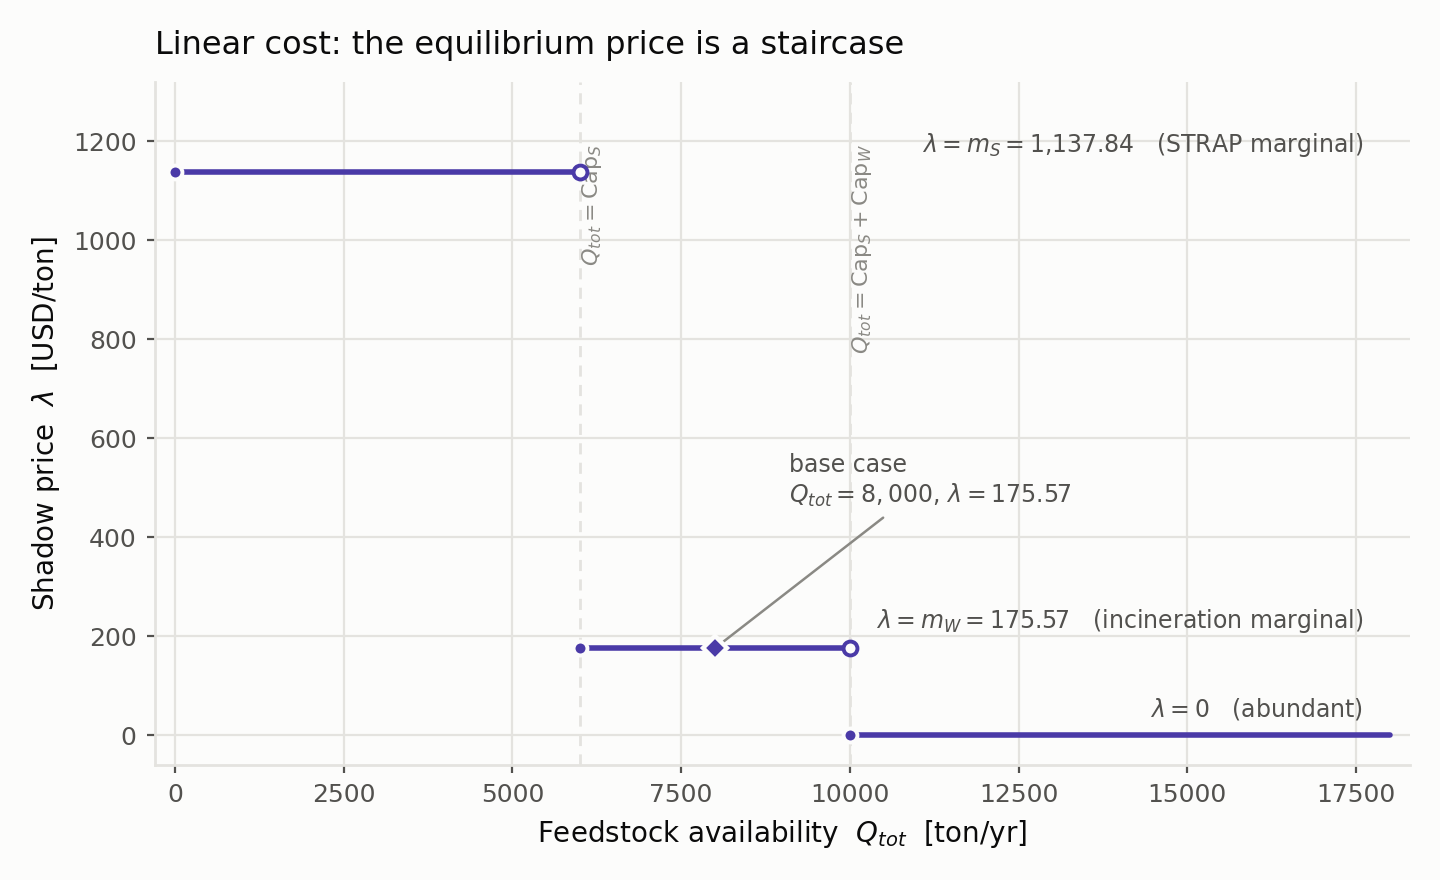
\includegraphics[width=0.92\textwidth]{figures/figL1_lambda_staircase.png}
\caption{Equilibrium shadow price $\lambda$ against feedstock availability.
Under linear cost the price is piecewise \emph{constant}: each tread is
attained at its left end (filled dot) and not at its right (open dot).}
\label{fig:L1}
\end{figure}

$\lambda$ takes exactly \textbf{three} values across the entire sweep
(Table~\ref{tab:sa1}). This is a direct consequence of linear cost: whichever
agent is on the margin has a \emph{constant} marginal cost, so it posts one
price and holds it for as long as it remains the marginal agent. The price
changes only when the marginal agent itself changes.

\begin{table}[h]
\centering
\caption{The three regimes of the linear-cost model. Each threshold is exact,
not numerical.}
\label{tab:sa1}
\begin{tabular}{@{}llrl@{}}
\toprule
Regime & $Q_{\mathrm{tot}}$ range [t/yr] & $\lambda$ [USD/t] & Who is on the margin \\
\midrule
Severe scarcity & $0 \leq Q_{\mathrm{tot}} < 6{,}000$ & $1{,}137.84$ & STRAP ($\lambda = m_S$) \\
Moderate scarcity & $6{,}000 \leq Q_{\mathrm{tot}} < 10{,}000$ & $175.57$ & Incineration ($\lambda = m_W$) \\
Abundance & $Q_{\mathrm{tot}} \geq 10{,}000$ & $0$ & Nobody; feedstock is landfilled \\
\bottomrule
\end{tabular}
\end{table}

\noindent Both thresholds are capacity sums, exactly:
\begin{align}
Q_{\mathrm{tot}} = \mathrm{Cap}_S &= 6{,}000 \text{ t/yr}
  &&\text{(STRAP saturates; price drops } 1{,}137.84 \to 175.57) \notag\\
Q_{\mathrm{tot}} = \mathrm{Cap}_S + \mathrm{Cap}_W &= 10{,}000 \text{ t/yr}
  &&\text{(incineration saturates; price drops } 175.57 \to 0) \notag
\end{align}
The \textbf{abundance threshold is exactly $10{,}000$ t/yr}, not $14{,}000$
(total installed capacity), because gasification's margin is negative
(Section~\ref{sec:opex}): its $4{,}000$ t/yr of capacity is never used at any
availability, so it contributes nothing to aggregate demand.

\subsubsection*{The price is not unique exactly at the two thresholds}

At $Q_{\mathrm{tot}} = 6{,}000$ every price in $[175.57,\,1{,}137.84]$ satisfies
all equilibrium conditions, and at $Q_{\mathrm{tot}} = 10{,}000$ every price in
$[0,\,175.57]$ does. Throughout this report, and in the code, the \emph{lowest}
consistent price is reported at those two points, which is why each tread of
Figure~\ref{fig:L1} is closed at its left end and open at its right.

\subsubsection*{The first jump is the striking one}

Just above $Q_{\mathrm{tot}} = \mathrm{Cap}_S$ the price falls by
$m_S - m_W = 962.27$ USD/ton --- an $85\%$ collapse --- in response to a
vanishingly small amount of extra feedstock. The economics are stark: below $6{,}000$ t/yr,
STRAP can absorb everything available, so it is the marginal buyer and
competition prices feedstock at \emph{STRAP's} willingness to pay. The moment
supply exceeds what STRAP can physically process, the marginal ton must go to
the next buyer in line, and incineration's willingness to pay is roughly
one-sixth of STRAP's. The price of feedstock is set entirely by whoever is
last in the queue, and that identity changes discontinuously.

\subsubsection*{Allocation: strict merit order}

\begin{figure}[h]
\centering
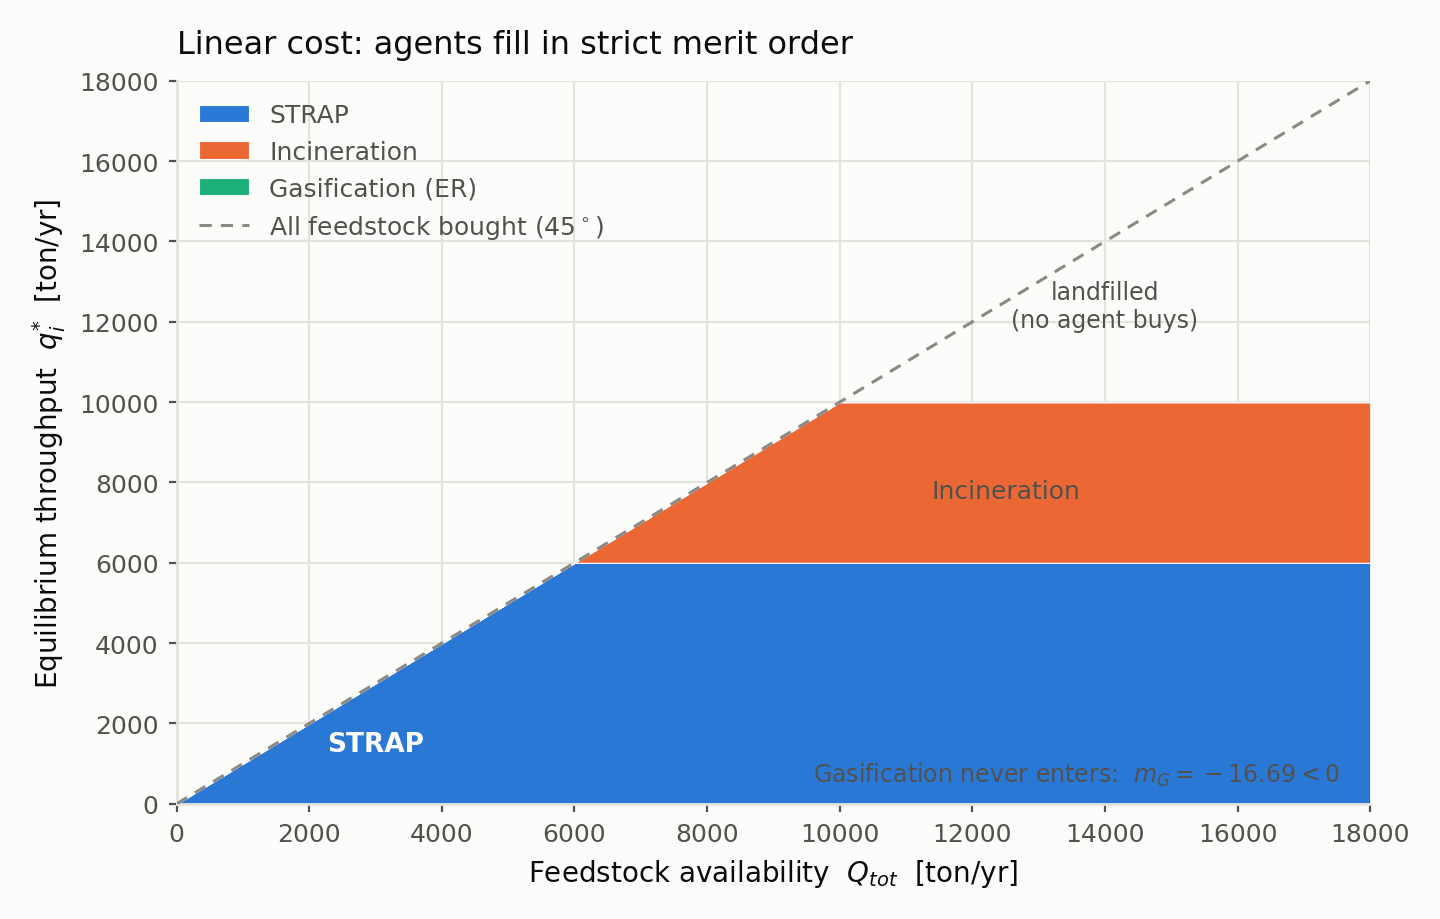
\includegraphics[width=0.92\textwidth]{figures/figL2_allocation.png}
\caption{Equilibrium allocation against availability. STRAP fills first, then
incineration; gasification never enters. Beyond $10{,}000$ t/yr the gap to the
$45^\circ$ line is feedstock nobody buys.}
\label{fig:L2}
\end{figure}

Agents fill in strict order of net margin, each running flat out before the
next one takes anything --- there is no range over which two agents share the
marginal ton. This is the same bang-bang structure as
Eq.~\eqref{eq:bestresponse}, seen from the quantity side.

\subsubsection*{What this does, and does not, tell us}

\textbf{What it establishes.} The merit order and both switching thresholds
are exact and robust: they depend only on the ranking of the margins $m_i$
and on the capacities, not on any curvature or shape assumption. The finding
that gasification never participates at \emph{any} feedstock level, and that
the market saturates at $10{,}000$ rather than $14{,}000$ t/yr, are real
results.

\textbf{What it cannot tell us.} Within a regime, $\lambda$ carries
\emph{no} information about how scarce feedstock actually is. At
$Q_{\mathrm{tot}} = 6{,}100$ t/yr (incineration barely started) and at
$9{,}900$ t/yr (incineration nearly saturated) the model returns the
identical price, $175.57$ USD/ton. A linear-cost model cannot express a
scarcity \emph{gradient} --- only scarcity \emph{regimes}. If the research
question is how sensitively the competitive price responds to marginal
changes in feedstock availability, this specification answers it with a flat
line inside each regime, and that is a limitation of the cost structure, not
of the equilibrium concept (see Section~\ref{sec:scope}).

\subsubsection*{Verification}

The sweep re-solves the equilibrium at $207$ points (200 evenly spaced, plus
each threshold and points a hair either side of it, plus the base case).
At every point:
\begin{itemize}[leftmargin=2em]
  \item every KKT and complementarity condition of
        Eqs.~\eqref{eq:kkt-q}--\eqref{eq:kkt-lambda} is satisfied with a
        worst residual of \textbf{exactly $0.0$} --- the merit-order solution
        is closed-form, so there is no iteration error to accumulate;
  \item $\lambda$ is non-increasing in $Q_{\mathrm{tot}}$, as an equilibrium
        price of a scarce good must be; and
  \item no two agents are ever simultaneously on the margin, so the
        degenerate-tie case of Section~\ref{sec:results-base} never arises
        and the allocation is unique at every swept point. The sweep raises
        rather than reports a result if it ever does.
\end{itemize}
Produced by \texttt{Code/linear\_model.py} and \texttt{Code/plots\_linear.py};
full numeric output in \texttt{Code/results/linear\_sweep\_q\_tot.csv}.


% =============================================================================
\section{Scope Boundaries}
\label{sec:scope}

The following are \textbf{deliberately excluded} from this version of the
model, and are not oversights:
\begin{itemize}[leftmargin=2em]
  \item \textbf{Convex operating cost.} Every agent's cost here is linear
        ($a_i q_i$). A convex (e.g.\ quadratic) refinement is a possible
        future extension, and SA-1 sharpens the case for it: it would
        (i) give $\lambda$ a genuine \emph{gradient} in $Q_{\mathrm{tot}}$
        rather than the flat treads of Figure~\ref{fig:L1}, so the model
        could distinguish mild from severe scarcity within a regime;
        (ii) let an agent's \emph{marginal} cost sit below its average cost
        at low throughput, which could let gasification enter the market
        despite $m_G < 0$ here; and (iii) remove the non-uniqueness noted in
        Section~\ref{sec:results-base} whenever two agents tie on margin.
        Not attempted in this draft.
  \item \textbf{Sensitivity work beyond SA-1.} Feedstock scarcity is swept in
        Section~\ref{sec:results-sa1}. Whether the assumed plant capacities
        are themselves defensible --- they set both thresholds in
        Table~\ref{tab:sa1}, so they matter more here than any other assumed
        input --- and how sensitive the headline number is to the most
        load-bearing assumed parameters are possible follow-on work, not
        attempted here.
  \item \textbf{Output-price coupling.} All product prices $P_k$ are fixed
        constants throughout; no agent's throughput affects market prices.
  \item \textbf{Cost coupling.} $c_{\mathrm{lf}}$ is a fixed parameter, not
        a function of total system-wide residue volume.
  \item \textbf{An emissions cap.} Emissions are computed and reported at
        the equilibrium but never constrain any agent's optimization.
  \item \textbf{Endogenous capacity / a two-stage capacity game.} The
        assumed capacities $\mathrm{Cap}_i$ are fixed inputs, not the
        outcome of a solved simultaneous-capacity equilibrium.
  \item \textbf{Any second shared constraint.} Exactly one shared feedstock
        constraint is used in this version.
\end{itemize}


% =============================================================================
\section{Questions for Paola}
\label{sec:questions}

The following ten questions concern parameters used in this model that are
not directly traceable to the paper, ranked roughly by how much each one
moves the headline result.

\begin{enumerate}[leftmargin=2em,itemsep=0.6em]

\item \textbf{Incineration operating cost.} The paper's own workbook records
      incineration OPEX and CAPEX as literally zero, because incineration is
      modeled only as a third-party off-take market (the planner \emph{sells}
      waste to it at 110 USD/ton), never as an owned, operated facility. This
      model assumed $75$ USD/ton, a mid-range figure for US municipal
      waste-to-energy O\&M. \emph{Do you have a per-ton operating-cost figure
      for incineration on this feedstock, or a reference you would trust?}

\item \textbf{Incineration revenue.} Two different numbers in the authors'
      own notebook could both plausibly be ``incineration revenue'':
      $\mathrm{Cwte} = 259.57$ USD/ton (listed alongside the STRAP resin
      prices as the value of the energy product) and $\mathrm{Cgas\_pw} =
      110$ USD/ton (the price the planner is paid for \emph{selling} waste
      to incineration). This model used $259.57$, reasoning that an
      operating firm earns the product value rather than a waste-transfer
      fee. \emph{Is $\mathrm{Cwte}$ the value of the energy product per
      tonne burned, and is $\mathrm{Cgas\_pw}$ the transfer price for the
      waste itself?} If these are reversed, incineration's margin falls
      from $175.57$ to $26.0$ USD/ton, a factor of about $6.8$.

\item \textbf{Assumed capacities.} $\mathrm{Cap}_S = 6{,}000$,
      $\mathrm{Cap}_W = \mathrm{Cap}_G = 4{,}000$ t/yr have no basis in the
      paper (only location Scenario 3's mention of a 20{,}000 t/yr
      \emph{shared} STRAP facility is suggestive). These values determine
      where the equilibrium price jumps as feedstock availability varies.
      \emph{Is there a defensible single-plant scale for STRAP, and any basis
      at all for incineration or gasification capacities?}

\item \textbf{Landfill tipping fee.} This model used $60$ USD/ton (a
      representative Wisconsin rate); the authors' own spreadsheet implies
      $7.836$ USD/ton, roughly $8\times$ lower than real gate rates.
      \emph{Is $7.836$ USD/ton really a tipping fee, or is it a different
      cost category (e.g.\ a per-ton \emph{processing} cost) that was
      mislabeled?}

\item \textbf{Capital recovery convention.} This model used a discounted
      10\%/20-year CRF (0.1175); the paper's own convention is undiscounted
      straight-line depreciation over 20 years (CRF $=0.05$). \emph{Was the
      undiscounted convention a deliberate choice?} (This affects which
      agents are viable net of capital, but never the equilibrium throughput
      or $\lambda$ itself.)

\item \textbf{Feedstock price.} This model assumed feedstock is free to every
      agent ($p_{\mathrm{raw}}=0$), matching the paper's treatment of its
      planner. The authors' own model separately implies a transfer price of
      110 USD/ton in a different context. Since $m_i$ shifts one-for-one
      with $p_{\mathrm{raw}}$ for every agent (Eq.~\eqref{eq:margin}),
      $\lambda$ would also move one-for-one with it, reaching zero around
      $p_{\mathrm{raw}} = 175.57$ USD/ton. \emph{What is the right feedstock
      price for a competitive multi-agent setting} --- is 110 USD/ton what a
      recycler would actually pay, or could post-industrial waste plausibly
      carry a \emph{negative} price (the generator pays to have it hauled
      away)?

\item \textbf{Residue/ash fractions.} The authors' spreadsheet records
      incineration and gasification ``Waste to Disposal'' as literally zero,
      which is not physically plausible. This model assumed $\rho_W = 0.15$
      and $\rho_G = 0.08$ ton/ton from standard ranges. \emph{Are the zero
      entries a placeholder, or is ash/char accounted for elsewhere in the
      original model?}

\item \textbf{Emissions table units.} Table 8's emissions column, headed
      ``kg CO$_2$-eq/year,'' reproduces exactly if the underlying factor is
      actually in \emph{tonnes} (Section~\ref{sec:parameters}).
      \emph{Can you confirm the Table 8/9/10 emissions columns are tonnes,
      not kilograms?}

\item \textbf{Table 8's profit figure.} This model's reconstruction of the
      max-profit pathway's cost from the authors' own per-wash CAPEX/OPEX
      data does not reproduce the published $7{,}551{,}142$ USD/yr under any
      single consistent accounting convention tested (shredder charged once
      vs.\ to both washes, wash-2 capital included or not).
      \emph{Which capital-accounting convention produced the published
      Table 8 figure?}

\item \textbf{Gasification revenue inputs.} The heat price ($0.13$ USD/MJ)
      and heat yield ($583$ MJ/tonne) used to compute gasification's revenue
      both look dimensionally unusual relative to typical industrial values.
      \emph{Are these in the units the notebook implies?}

\end{enumerate}


% =============================================================================
\section*{References}
\addcontentsline{toc}{section}{References}

\noindent Mu\~{n}oz-Briones, P.; Ikegwu, U.\ M.; Martinez, K.\ J.; Granger,
C.; Van Lehn, R.\ C.; Zavala, V.\ M.; Huber, G.\ W.; Avraamidou, S.
\emph{Decision support for circular economy waste management of mixed
plastic streams: A case study on post-industrial multilayer films.}
(Paper on file, \texttt{Paola\_Game\_Theory/\allowbreak Paper/}.)

\end{document}
